\begin{apendicesenv}
\partapendices
\chapter{Cronograma}
\label{sec:cronograma}
\FloatBarrier
\begin{figure}[!htpd]
		\centering
		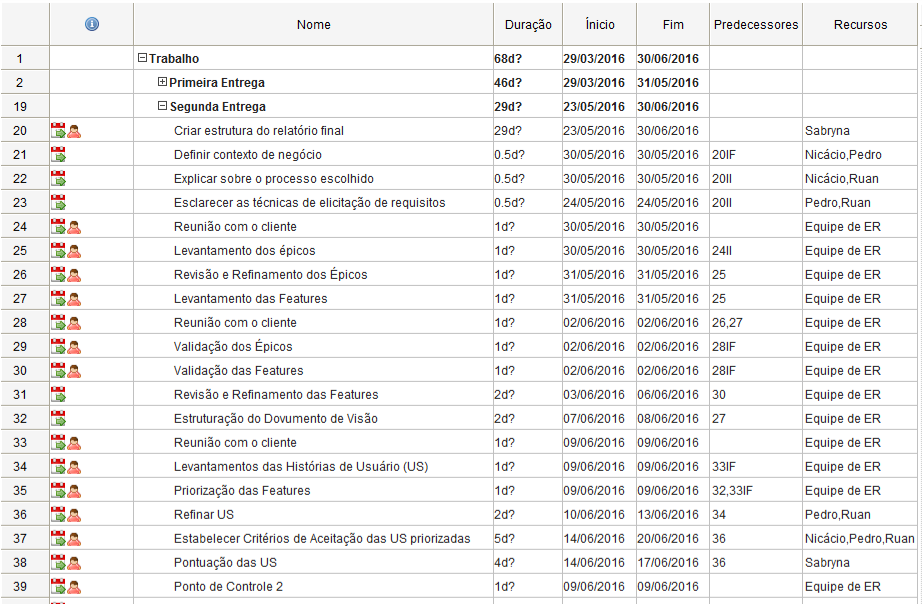
\includegraphics[scale=0.5]{figuras/cron1}
		\label{img:cronograma}
		\caption{Cronograma de Atividades}
\end{figure}
\FloatBarrier

\FloatBarrier
\begin{figure}[!htpd]
		\centering
		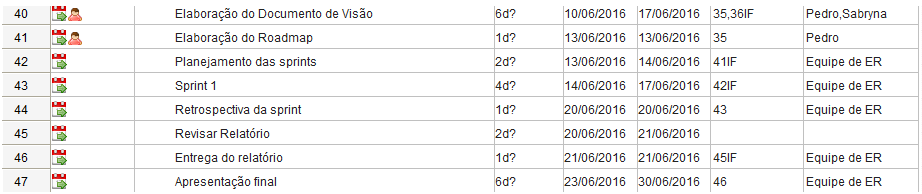
\includegraphics[scale=0.5]{figuras/cron2}
		\label{img:cronograma}
		\caption{Cronograma de Atividades}
\end{figure}
\FloatBarrier

\chapter{Processo de Engenharia de Requisitos}
\label{sec:processo}
\FloatBarrier
\begin{figure}[!htpd]
		\centering
		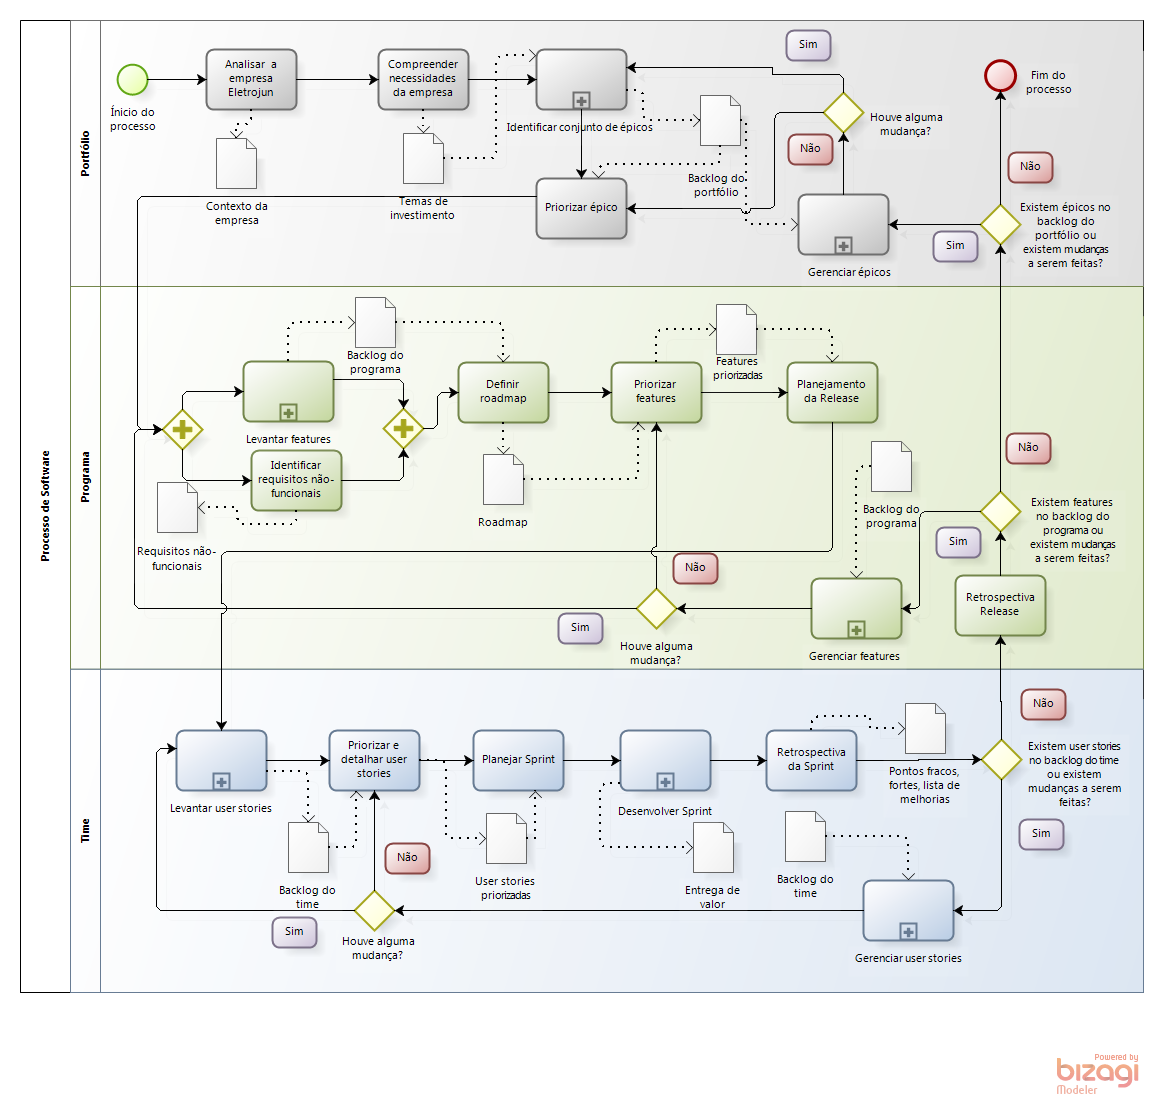
\includegraphics[scale=0.55]{figuras/Eletrojun}
		\label{img:processoeletrojun}
		\caption{Visão geral do processo}
\end{figure}
\FloatBarrier

\chapter{Documento de Visão}
\label{sec:visão}

\textbf{Histórico de Revisões}

\FloatBarrier
\begin{table}[!htpd]
\centering
\label{my-label}
\begin{tabular}{|l|l|l|l|}
\hline
Versão & Data  & Descrição      & Autor(es)                                                                                                \\ \hline
0.5    & 11/06 & Versão Inicial & \begin{tabular}[c]{@{}l@{}}Nicácio Arruda, Pedro Sales, Ruan Herculano,\\  Sabryna de Sousa\end{tabular} \\ \hline
1.0    & 15/06 & Finalização    & \begin{tabular}[c]{@{}l@{}}Nicácio Arruda, Pedro Sales, Ruan Herculano,\\  Sabryna de Sousa\end{tabular} \\ \hline
\end{tabular}
\end{table}

\section{Introdução}

Este documento aborda as características do sistema de Compartilhamento de Projetos, trazendo uma visão do sistema como um tudo, relatando as funcionalidades, o problema que inicial e a solução a ser desenvolvida.

\subsection{Finalidade}

A principal finalidade deste documento é trazer uma visão clara e uma especificação preliminar do software para todos os envolvidos e beneficiários da execução deste.

\subsection{Escopo}

O escopo deste documento visa tornar claro a definição dos requisitos do sistema de compartilhamento de projetos, sendo utilizado a abordagem do SAFe para a elicitação dos mesmos.

\subsection{Visão Geral}

Este documento de visão mostra uma breve introdução sobre o sistema, seguido do posicionamento, onde são abordados os problemas e as motivações para criar este produto. Ele esclarece quem são os envolvidos e  apresenta uma visão geral do produto.

\section{Posicionamento}

\subsection{Oportunidade de Negócios}

A empresa Eletrojun pretende ampliar a sua rede de conexões entre alunos, buscando criar um sistema que auxilie todos da Universidade de Brasília. O principal objetivo deste sistema é a interação entre os usuários do mesmo, a fim de criar uma rede colaborativa em que as pessoas colocam suas ideias, projetos e recebem ajuda de outras pessoas, podendo até mesmo vender suas ideias e inserir um produto no mercado.

\subsection{Descrição do Problema}

\FloatBarrier
\begin{table}[!htpd]
\centering
\caption{Descrição do problema}
\label{my-label}
\begin{tabular}{|l|l|}
\hline
O problema de         & Falta de compartilhamento de projetos                                                                                                                                                                                                                                                                                                                                                            \\ \hline
afeta                 & os alunos da Universidade de Brasília                                                                                                                                                                                                                                                                                                                                                            \\ \hline
cujo impacto é        & \begin{tabular}[c]{@{}l@{}}falta de conhecimento por parte dos interessados em colaborar com\\ projetos sobre a existência e o andamento destes, bem como a falta \\ de integração e organização na administração de projetos dos alunos\end{tabular}                                                                                                                                            \\ \hline
uma boa solução seria & \begin{tabular}[c]{@{}l@{}}criar um sistema que pudesse juntar todas as funcionalidades de \\ publicar um projeto, receber ajuda para o desenvolvimento de uma ideia,\\ saber o status de uma atividade, ter uma rede de amigos colaboradores, \\ vender um produto ou uma ideia com ajuda de demais participantes, e ter \\ uma integração dos alunos da Universidade de Brasília.\end{tabular} \\ \hline
\end{tabular}
\end{table}

\subsection{Sentença de Posição do Produto}

\FloatBarrier
\begin{table}[!htpd]
\centering
\caption{Sentença de posição do produto}
\label{my-label}
\begin{tabular}{|l|l|}
\hline
Para                                                                                 & os alunos da Universidade de Brasília                                                                                                                                                                                                                                                                                                        \\ \hline
Que                                                                                  & necessitam de uma rede colaborativa                                                                                                                                                                                                                                                                                                          \\ \hline
\begin{tabular}[c]{@{}l@{}}O sistema de compartilhamento \\ de projetos\end{tabular} & é uma rede                                                                                                                                                                                                                                                                                                                                   \\ \hline
Que                                                                                  & \begin{tabular}[c]{@{}l@{}}contém funcionalidades de interação de usuários, administração\\ e compartilhamento de projetos em uma plataforma web\end{tabular}                                                                                                                                                                                \\ \hline
Diferente de                                                                         & Trello, Google Drive, Kickstarter, Instructables                                                                                                                                                                                                                                                                                             \\ \hline
Nosso produto                                                                        & \begin{tabular}[c]{@{}l@{}}tem todas funcionalidades para gestão de um projeto, podendo \\ ser compartilhado com diversos amigos, vendido, ter status\\ sobre o seu progresso e visibilidade, centralizando todas as \\ funcionalidades que necessitariam de diversas plataformas para\\  serem supridas, em uma só plataforma.\end{tabular} \\ \hline
\end{tabular}
\end{table}
\FloatBarrier

\section{Envolvidos e Usuários}

\subsection{Envolvidos}

\FloatBarrier
\begin{table}[!htpd]
\centering
\caption{Envolvidos no sistema}
\label{my-label}
\begin{tabular}{|l|l|l|}
\hline
Nome                                                                                 & Descrição                                                                              & Responsabilidades                                                                                                                                              \\ \hline
Mônica                                                                               & \begin{tabular}[c]{@{}l@{}}Diretora da empresa \\ Eletrojun\end{tabular}               & \begin{tabular}[c]{@{}l@{}}Assegurar que os objetivos do software sejam \\ atendidos.\\ Monitorar o projeto\\ Aprovar novas ideias para o sistema\end{tabular} \\ \hline
\begin{tabular}[c]{@{}l@{}}Analistas de Requisitos \\ e Desenvolvedores\end{tabular} & \begin{tabular}[c]{@{}l@{}}Alunos da disciplina\\  Requisitos de Software\end{tabular} & \begin{tabular}[c]{@{}l@{}}Elicitar requisitos \\ Desenvolver parcialmente o sistema\end{tabular}                                                              \\ \hline
\end{tabular}
\end{table}
\FloatBarrier

\subsection{Usuários}

Os usuários da plataforma serão os alunos do Campus Gama da Universidade de Brasília que venham a ter interesse na criação de projetos, visando ter um controle administrativo de colaboradores e tarefas, além de torná-lo visado e comercializável. Também é destinado aos alunos que sejam interessados em contribuir com projetos em andamento.

Os perfis de usuário do sistema são caracterizados por:

\FloatBarrier
\begin{table}[!htpd]
\centering
\caption{Usuários do sistema}
\label{my-label}
\begin{tabular}{|l|l|}
\hline
Nome                     & Descrição                                                                                                                                    \\ \hline
Usuário do sistema       & \begin{tabular}[c]{@{}l@{}}Usuário que pode criar projetos, tarefas, conversar no chat com \\ seus amigos\end{tabular}                       \\ \hline
Usuário colaborador      & \begin{tabular}[c]{@{}l@{}}Usuário responsável pela execução de tarefas e colaborações com \\ os projetos\end{tabular}                       \\ \hline
Gerente de projeto       & \begin{tabular}[c]{@{}l@{}}Usuário responsável pela administração e distribuição de \\ atividades dos projetos\end{tabular}                  \\ \hline
Administrador do sistema & \begin{tabular}[c]{@{}l@{}}Usuário responsável por manter a plataforma, bem como controle \\ de usuários e projetos cadastrados\end{tabular} \\ \hline
\end{tabular}
\end{table}

\subsubsection{Ambiente dos Usuários}

Todos os usuários da plataforma poderão acessá-la por acesso à internet, via browser de sua preferência por meio do website oficial, utilizando para tal tanto computadores quanto aparelhos mobile.

\section{Visão Geral do Produto}

O sistema consiste num website para auxiliar o desenvolvimento de projetos acadêmicos. Este sistema possibilita que os estudantes compartilhem ideias de projetos e outras informações relevantes sobre o assunto. Os usuários podem contribuir com os projetos existentes de várias formas e podem executar tarefas dentro destes projetos, sendo premiado com moedas do sistema. Os melhores projetos participam de um ranking de projetos onde os usuários podem votar e escolher entre os projetos disponíveis, corroborando para a divulgação do mesmo, de forma a facilitar e propiciar a comercialização. O criador do projeto no sistema pode convidar membros para o projeto e criar atividades. Há também um sistema de chat que possibilita a comunicação entre os usuários.

\section{Épicos}

Analisando a solução em nível macro, foram especificados quatro épicos que abrangessem todo o contexto da proposta, delimitando as fronteiras do problema a ser resolvido. Estes são:

\textbf{Épico 01 - EP-01:} Gerenciamento de Usuários: Abrange todas as ações de administração dos usuários do sistema, desde o cadastro de um usuário até a sua exclusão do sistema.

\textbf{Épico 02 - EP-02:} Gerenciamento de Projetos: Abrange todas as ações de administração de projetos no sistema, desde a sua publicação até o seu cumprimento total.

\textbf{Épico 03 - EP-03:} Gerenciamento de Atividades: Abrange todas as ações de administração e gerenciamento de atividades pontuais, dentro e fora dos projetos.

\textbf{Épico 04 - EP-04:} Gerenciamento de Premiações: Abrange todas as ações manutenção de premiações aos usuários do sistema.

\section{Features}

A partir dos Épicos, foram levantadas e priorizadas as Features fundamentais, de acordo com a seguinte tabela:

\FloatBarrier
\begin{table}[!htpd]
\centering
\caption{Features priorizadas}
\label{my-label}
\begin{tabular}{|l|l|l|}
\hline
\textbf{Épico} & \textbf{Features}                  & \textbf{Descrição}                                                                                                                                    \\ \hline
Épico 1        & Feature 1 - Manutenção de Usuários & \begin{tabular}[c]{@{}l@{}}Esta feature tem como objetivo manter \\ os usuários do sistema, permitindo o \\ cadastro e edição de perfil.\end{tabular} \\ \hline
Épico 1        & Feature 2 - Acesso dos Usuários    & \begin{tabular}[c]{@{}l@{}}Esta feature é responsável pelo controle \\ de acesso dos usuários, que podem \\ realizar o login e o logout.\end{tabular} \\ \hline
Épico 1        & Feature 3 - Manutenção de projetos & \begin{tabular}[c]{@{}l@{}}Feature responsável pelo cadastro, \\ edição, e exclusão de projetos.\end{tabular}                                         \\ \hline
Épico 1        & Feature 11- Sistema de tarefas     & \begin{tabular}[c]{@{}l@{}}Feature responsável por especificar e \\ controlar atividades designadas aos \\ usuários do projeto.\end{tabular}          \\ \hline
\end{tabular}
\end{table}
\FloatBarrier

\section{Histórias de Usuário}

Dentro das Features priorizadas foram selecionadas ainda as Histórias de Usuário priorizadas.

\FloatBarrier
\begin{table}[!htpd]
\centering
\caption{Histórias de Usuário priorizadas}
\label{my-label}
\begin{tabular}{|l|l|l|}
\hline
\textbf{Feature} & \textbf{Histórias de Usuário} & \textbf{Descrição}                                                                                                                                                                           \\ \hline
Feature 1        & US1                           & \begin{tabular}[c]{@{}l@{}}Eu como usuário, quero cadastrar-me no \\ sistema de compartilhamento de projetos.\end{tabular}                                                                   \\ \hline
Feature 1        & US2                           & \begin{tabular}[c]{@{}l@{}}Eu como usuário, quero alterar meus dados \\ cadastrais para manter meu cadastro atualizado.\end{tabular}                                                         \\ \hline
Feature 1        & US3                           & \begin{tabular}[c]{@{}l@{}}Eu como usuário, quero excluir minha conta \\ para não ser mais usuário do sistema.\end{tabular}                                                                  \\ \hline
Feature 2        & US4                           & \begin{tabular}[c]{@{}l@{}}Eu como usuário, quero fazer login no sistema \\ de compartilhamento de projetos para,acessar \\ o sistema.\end{tabular}                                          \\ \hline
Feature 2        & US5                           & \begin{tabular}[c]{@{}l@{}}Eu como usuário, quero fazer logout no sistema \\ para sair do sistema e encerrar a sessão.\end{tabular}                                                          \\ \hline
Feature 3        & US8                           & \begin{tabular}[c]{@{}l@{}}Eu como criador de projeto, quero criar um \\ projeto para para que ele possa ser desenvolvido \\ no sistema.\end{tabular}                                        \\ \hline
Feature 3        & US9                           & \begin{tabular}[c]{@{}l@{}}Eu como criador do projeto, quero remover um \\ projeto para interromper/impedir o seu \\ desenvolvimento no sistema.\end{tabular}                                \\ \hline
Feature 3        & US10                          & \begin{tabular}[c]{@{}l@{}}Eu como criador de projeto, quero editar os dados \\ do projeto para corrigir algum erro de digitação, \\ ou refinar os dados cadastrais do projeto.\end{tabular} \\ \hline
Feature 3        & US33                          & \begin{tabular}[c]{@{}l@{}}Eu como criador do projeto, quero manter tarefas \\ para que os contribuidores possam contribuir \\ com elas.\end{tabular}                                        \\ \hline
\end{tabular}
\end{table}
\FloatBarrier

\chapter{Roadmap}
\label{sec:roadmap}
\FloatBarrier
\begin{figure}[!htpd]
		\centering
		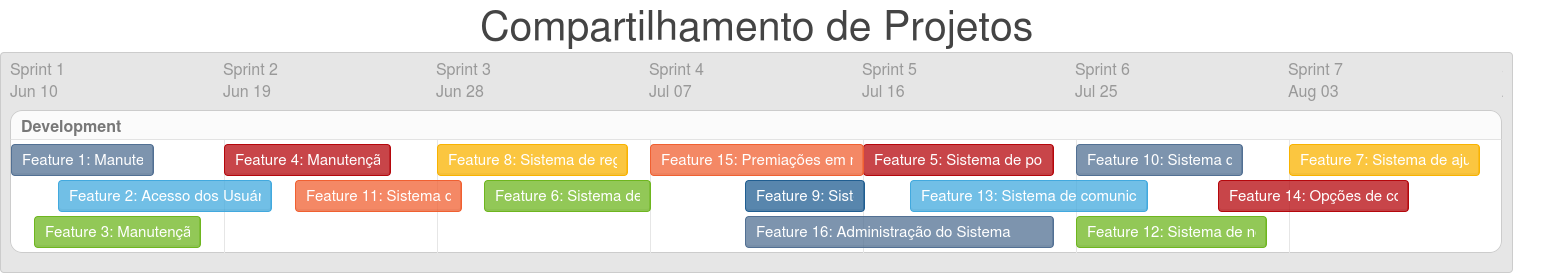
\includegraphics[scale=0.3]{figuras/roadmap}
		\label{img:roadmap}
		\caption{Roadmap completo}
\end{figure}

\chapter{Atas de Reuniões}

\section{Reunião 1}

\subsection{Documento}

\FloatBarrier
\begin{table}[!htpd]
\centering
\label{my-label}
\begin{tabular}{|l|l|}
\hline
\multicolumn{2}{|l|}{Projeto/Release: Gerenciamento e Compartilhamento de Projetos} \\ \hline
Coordenador: Mônica Damasceno                  & Arquivo/Versão: 1                  \\ \hline
\multicolumn{2}{|l|}{Data da preparação: 28/04/2016}                                \\ \hline
\end{tabular}
\end{table}
\FloatBarrier

\subsection{Reunião}

\FloatBarrier
\begin{table}[!htpd]
\centering
\label{my-label}
\begin{tabular}{|l|l|l|}
\hline
Data da reunião: 30/05/2016 & Horário: 18:00 & \begin{tabular}[c]{@{}l@{}}Local: FGA (Faculdade UnB Gama),\\ em frente a biblioteca.\end{tabular} \\ \hline
\multicolumn{3}{|l|}{Objetivo da reunião: Obter uma noção geral do sistema}                                                                       \\ \hline
\end{tabular}
\end{table}
\FloatBarrier

\subsection{Participantes da reunião}

\FloatBarrier
\begin{table}[!htpd]
\centering
\label{my-label}
\begin{tabular}{|l|}
\hline
\textbf{Nome}             \\ \hline
Ruan N. Herculano Pereira \\ \hline
Sabryna de Sousa             \\ \hline
Nicacio Arruda            \\ \hline
Mônica Damasceno          \\ \hline
Pedro Sales               \\ \hline
\end{tabular}
\end{table}
\FloatBarrier

\subsection{Pauta}
Obter uma visão geral do sistema, bem como compreender o contexto que a empresa se encontra, suas necessidades e entender o motivo para a construção do sistema, bem como os problemas que a mesma busca solucionar

\subsection{Decisões}
Foram levantados os principais problemas a serem sanados, além do contexto em que a empresa em questão se insere. Foram decididos os temas de negócio e o levantamento inicial dos épicos que abrangem a solução.

\subsection{Considerações finais}

Foi possível realizar o primeiro contato com o cliente, de forma a extrair informações de seus objetivos e assim, estabelecer um contato produtivo e centrado na solução dos problemas.

\section{Reunião 2}

\subsection{Documento}

\FloatBarrier
\begin{table}[!htpd]
\centering
\label{my-label}
\begin{tabular}{|l|l|}
\hline
\multicolumn{2}{|l|}{Projeto/Release: Gerenciamento e Compartilhamento de Projetos} \\ \hline
Coordenador: Mônica Damasceno                  & Arquivo/Versão: 1                  \\ \hline
\multicolumn{2}{|l|}{Data da preparação: 01/06/2016}                                \\ \hline
\end{tabular}
\end{table}
\FloatBarrier

\subsection{Reunião}

\FloatBarrier
\begin{table}[!htpd]
\centering
\label{my-label}
\begin{tabular}{|l|l|l|}
\hline
Data da reunião: 01/06/2016 & Horário: 18:00 & \begin{tabular}[c]{@{}l@{}}Local: FGA (Faculdade UnB Gama),\\ em frente a biblioteca.\end{tabular} \\ \hline
\multicolumn{3}{|l|}{Objetivo da reunião: Obter uma noção geral do sistema}                                                                       \\ \hline
\end{tabular}
\end{table}
\FloatBarrier

\subsection{Participantes da reunião}

\FloatBarrier
\begin{table}[!htpd]
\centering
\label{my-label}
\begin{tabular}{|l|}
\hline
\textbf{Nome}             \\ \hline
Ruan N. Herculano Pereira \\ \hline
Sabryna de Sousa             \\ \hline
Nicacio Arruda            \\ \hline
Mônica Damasceno          \\ \hline
Pedro Sales               \\ \hline
\end{tabular}
\end{table}
\FloatBarrier

\subsection{Pauta}
Esta reunião tem o objetivo de validar os épicos e e as features levantadas de acordo com o que foi obtido e executado a partir da reunião anterior, de forma a alinhar com o cliente se as necessidades estão sendo abordadas de forma adequada.

\subsection{Decisões}
Foi alinhado com o cliente e planejado a refatoração das features, utilizando a técnica de brindstorm para melhor elicitar as necessidades reais do cliente. Foi também feito o alinhamento e validação dos épicos preveamente descritos e levantados.

Também foi analisado o projeto já iniciado, de forma a validar as correções e alinha-las com os requisitos já elicitados, de forma a manter a concisão da solução com o sistema pré desenvolvido, levantando as correções necessárias a este.

\subsection{Considerações finais}

Foi possível aproximar ainda mais as ideias do cliente para o contexto da aplicação, de forma a tornar o caminho até a solução ainda mais claro.

\section{Reunião 3}

\subsection{Documento}

\FloatBarrier
\begin{table}[!htpd]
\centering
\label{my-label}
\begin{tabular}{|l|l|}
\hline
\multicolumn{2}{|l|}{Projeto/Release: Gerenciamento e Compartilhamento de Projetos} \\ \hline
Coordenador: Mônica Damasceno                  & Arquivo/Versão: 1                  \\ \hline
\multicolumn{2}{|l|}{Data da preparação: 08/06/2016}                                \\ \hline
\end{tabular}
\end{table}
\FloatBarrier

\subsection{Reunião}

\FloatBarrier
\begin{table}[!htpd]
\centering
\label{my-label}
\begin{tabular}{|l|l|l|}
\hline
Data da reunião: 09/06/2016 & Horário: 18:00 & \begin{tabular}[c]{@{}l@{}}Local: FGA (Faculdade UnB Gama),\\ em frente a biblioteca.\end{tabular} \\ \hline
\multicolumn{3}{|l|}{Objetivo da reunião: Obter uma noção geral do sistema}                                                                       \\ \hline
\end{tabular}
\end{table}
\FloatBarrier

\subsection{Participantes da reunião}

\FloatBarrier
\begin{table}[!htpd]
\centering
\label{my-label}
\begin{tabular}{|l|}
\hline
\textbf{Nome}             \\ \hline
Ruan N. Herculano Pereira \\ \hline
Sabryna de Sousa             \\ \hline
Nicacio Arruda            \\ \hline
Mônica Damasceno          \\ \hline
Pedro Sales               \\ \hline
\end{tabular}
\end{table}
\FloatBarrier

\subsection{Pauta}
Esta reunião tem como objetivo explicitar e validar tudo o que foi levantado até o momento, de forma a manter a solução consida. Também se faz necessária nesta reunião o levantamento prévio das Histórias de Usuário com o cliente, de forma a aprofundar o entendimento da aplicação por meio da técnica de brindstorm.

Após o levantamento das histórias, teremos argumentos suficientes para a priorização das features e suas histórias, de forma a elucidar a importância de cada processo descrito para a solução geral, e podendo ser planejado em seguida a execução da primeira release

\subsection{Decisões}
Assim como planejado, foi evidenciado ao cliente todo o material de requisitos produzido até o presente momento e levantadas as histórias de usuário com o mesmo. Após o levantamento, foi feito uma priorização das features e histórias de usuário.

Iniciou-se também o levantamento dos critérios de aceitação para as histórias levantadas, ficando para executar a completude da atividade a distância.

\subsection{Considerações finais}
Apesar de ter sido uma reunião densa em atividades executadas, devido a sincronia obtida entre a equipe de Engenharia de Requisitos e o cliente, ainda com a ajuda da efetividade das técnicas adotas, pode-se elicitar uma grande quantidade de conteúdo e material para o planejamento e início da primeira release do projeto.

\end{apendicesenv}
